\section{Introduction}
\subsection{Project Aims, Objectives and Introduction} 
Phil Beadle \cite{website:TES} explains in his article why the seating plan is the single most important piece of behavioural modification equipment in a teachers toolbox. Phil lays more emphasis on how the way pupils sit in the classroom impacts their learning and their participation in the classroom. A survey of students asking them ``How do they learn best?'' made it clear that students learn best in groups, as they all replied they work better in groups.

Teachers have a wide range of tools and software applications to aide them with their daily tasks and most of these software suites come with a classroom seating feature but these tools are developed with a one size fits all ideology.There is research that lays out how best to group students in a classroom but since almost all the tools teachers have at their disposal are rigid with no flexibility they cannot experiment with these research findings to the better of their students.

Teachers are known to take matters in their hands by performing seating arrangements on a piece of paper or worse not bother with the extra work but go with the default structure to the detriment of the students.

A better way to solve this and to encourage teachers to experiment with proven findings on how to get the best out of students in a classroom would be to develop a web application that helps them with seating arrangements and one with an \emph{Adaptive User Interface} and breaks away from the one size fits all ideology to a one size fits none ideology. Where the interface can make implicit inference on how the system is being used and how best to help the user complete their tasks.

The notion of Adaptive User Interfaces has been around for several years, gathering an enormous amount of interest in the research community. Over the years a lot of technological advancements have been made in addition to standards and techniques to achieve adaptiveness on the user facing or interface layer of software applications. Example [interbook@Aha]. \cite{brusilovsky2007user} 

An adaptive user interface monitors the users activity trying to identify usage patterns and automatically adjust the interface components or content provided by the system to accommodate such user differences as well as changes in user skills, knowledge and preferences.\cite{alvarez2007current}

This can be achieved through a number of approaches; namely Task models, User Models and Artificial Intelligence Techniques. This project utilises User Model Technique. 

User models are used to generate or adapt user interfaces at runtime, to address particular user needs and preferences. User models are also known as user profiles, personas or archetypes. The user preferences and needs are represented by variables \cite{W3C}.

This project aims to use the User Model approach to develop a web application with an \emph{Adaptive User Interface} that teachers can use to manage their classrooms in terms of seating pairing and arrangement of pupils. The underlying User Model of the application is based on research findings on how to best group students in a classroom:

\begin{itemize}
    \item Groups - A general rule that applies to the application domain (seating plan); students work better in groups.
    \item Boys and Girls together - A general rule of pairing boys and girls together ; boys work better when paired with girls with a slightly lower ability. \cite{OFSTED}
    \item Current Context - that is, the current highly rated seating pattern by the teacher. 
\end{itemize}

The figure below \ref{fig:User-Model} illustrates the overview of the system and what it does. Teachers import student data in a Comma Separated Values format this forms part of the teachers user data. If the teacher is a returning user then any previously used seating plan rated highly by the user forms part of his or her user data. if the user is new then this variable is populated with the default which obeys the first two of the rules mentioned in the previous paragraph.

The adaptation effect is achieved by implicitly identifying patterns in the seating plans favoured by the user( highly rated previously used plans), although the system requires the user to explicitly score the plans they use based on its effectiveness and how the students responded. The User Model algorithm alters its rules based on these patterns. Example a teacher despite the research indicating boys work best with slightly lower ability girls may have his or her most effective seating plan being one where boys are paired together with other boys. The UM algorithm would identify this and then change its rules to reflect this, that is to reflect the teachers preferences.

The adaptation rule is initially applied when the teacher uses the system for the first time, the default rule is applied this time as the system does not have any history of seating plans to work with. The effect is evident when the user moves a student around in the classroom space, if a pairing is the best as specified by the current rule they are highlighted green and if it is the worse they are highlighted red. These adaptations are in the form of recommendations - the user does not necessarily have to follow this, they can override and form their own seating rules by telling the system how effective their rules ( seating pairing) are.


\begin{figure}[!ht]
\caption{User Modeling Overview}
    \label{fig:User-Model}
    \centering
    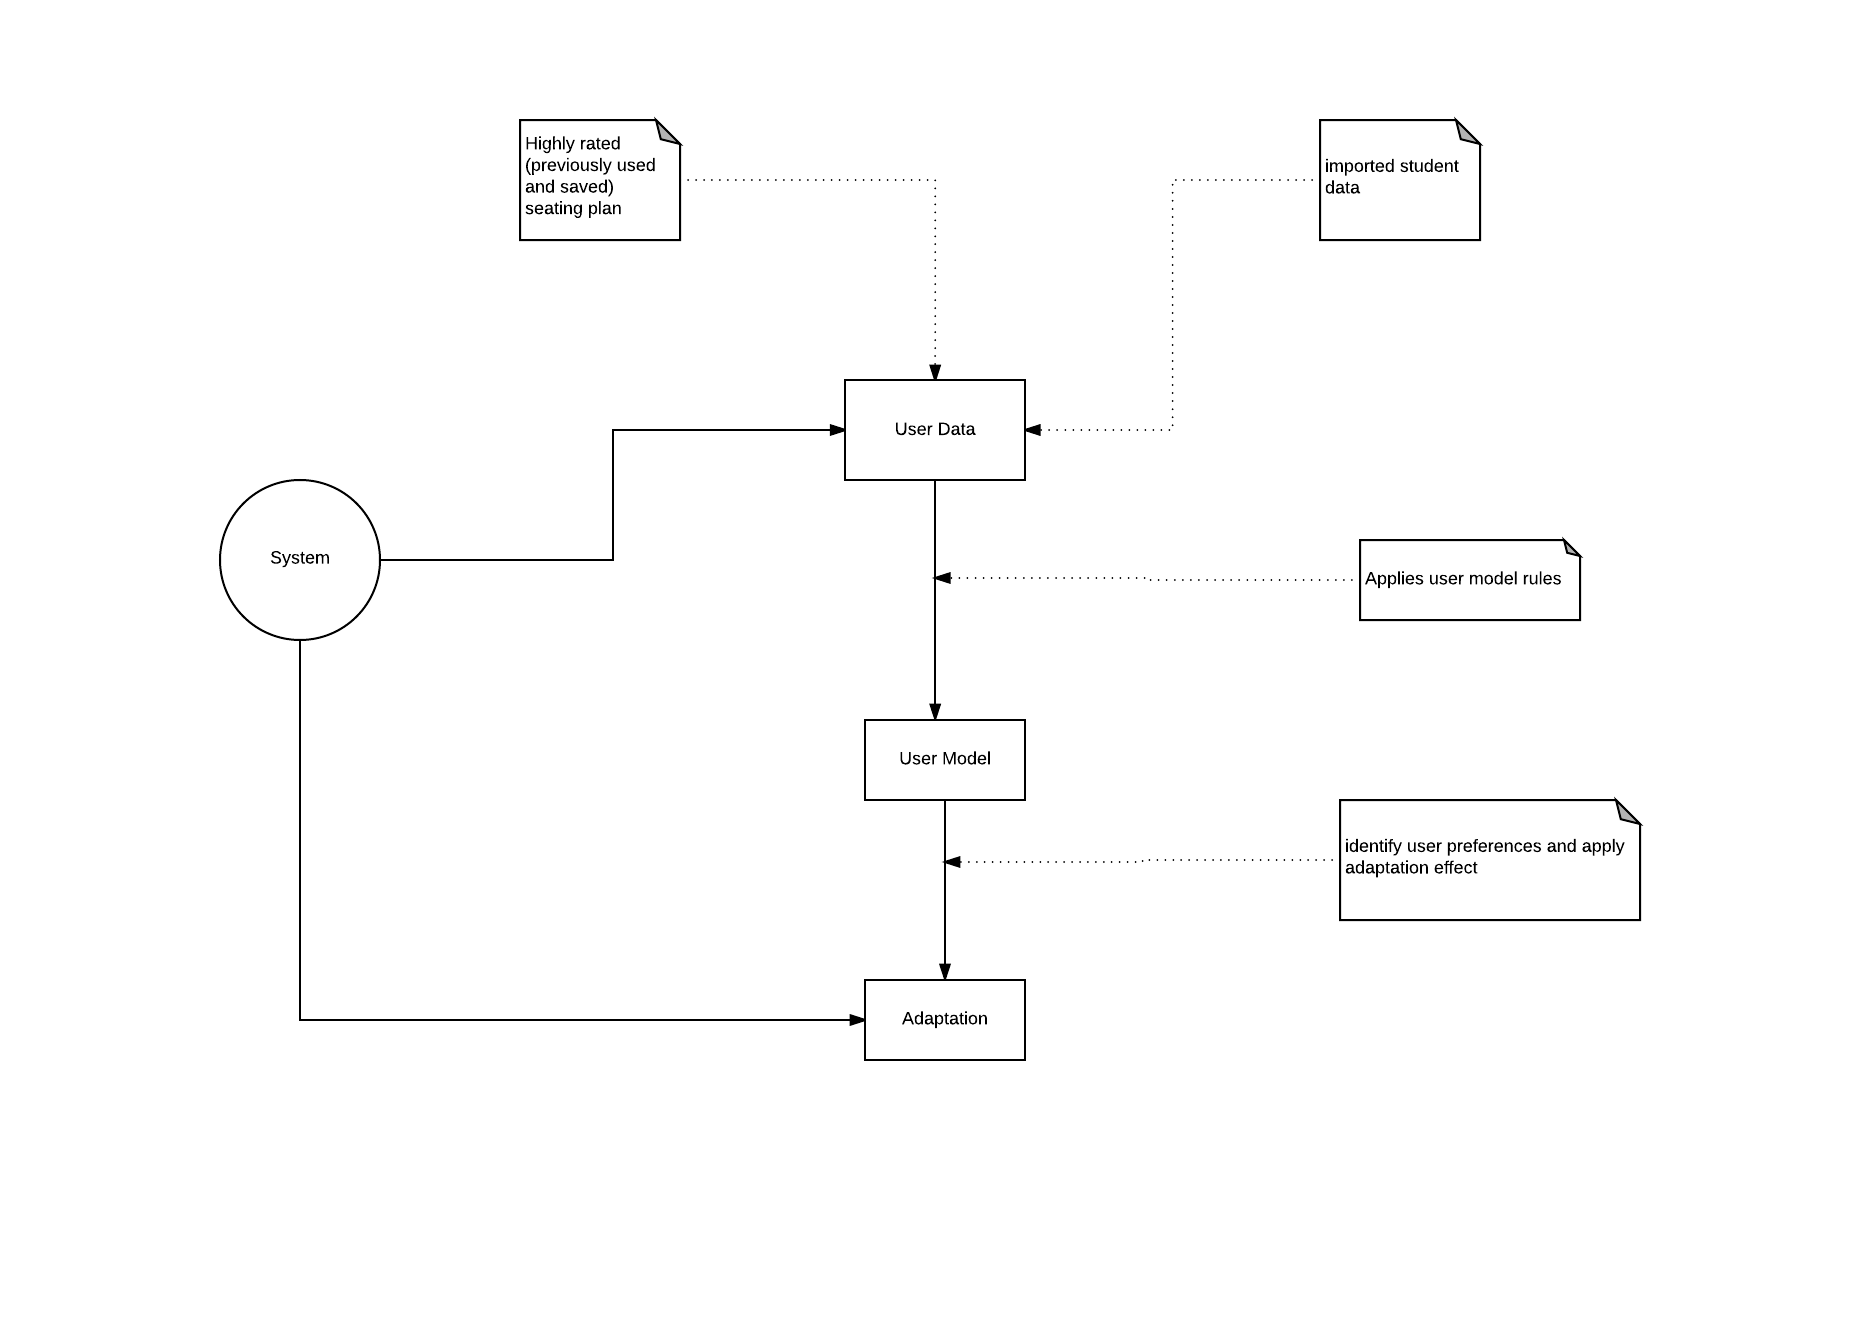
\includegraphics[scale=0.5]{figures/UM_Overview}
\end{figure}

The main components of the system are classroom space( canvas ) on which students are rendered, a history stack (holding references) to all seating plans used by the user and a User Model algorithm that identify usage patterns and apply adaptation rules respectively. We will discuss the implementation and design in detail in the next chapters.

In chapter two of this paper we will look at and critically discuss existing approaches to classroom management or behavioural tools and existing classroom management tools and or systems under literature review.

Chapter 3 looks at the design requirements of the system in detail, discussing the non-functional and functional requirements as well as user requirements of the system.

We will talk about the implementation of the overall system and the architecture as well as design patterns adopted in chapter 4. We will discuss the User Model algorithm in detail as well as show some code snippets of relevant methods that play a critical part in providing the user with the right adaptation effect.


\subsection{Background and Literature Survey} \label{sub:background}
In its salient form, an adaptive user interface or system monitors the users interaction with the system or interface and then tries to identify a pattern in the system's usage attributed to user difference s in order to automatically adjust the interface components or content to allow for such user differences as awell as changes in user skills, knowledge and preferences.

We see examples of such mechanisms in our daily usage of our smart phones, laptops and or on our favourite social media platforms. Facebook's advertising feature shows products unique to users based on what their adaptive system has identified as a pattern associated to the user.On our smartphones, features like the predictive text is a form of adaptiveness. It learns and tries to improve a users texting or typing experience.
\subsubsection{A brief history of user interfaces} \label{sub:history}
The concept of \emph{user interfaces} surfaced in the 1960's, when in 1963 Ivan Sutherland published his MIT PhD thesis about a system called \textbf{Sketchpad} \cite{sutherland1964sketch}.
The result of Ivan Sutherland's Sketchpad was a pioneering graphical user interface (GUI) and direct manipulation system. Sketchpad allowed the user to create graphic images directly on the computer screen using a lightpen \cite{patrick2003intelligent}.
Prior to the early 1970's, researchers focused primarily on new technologies but this trend changed in 1970 when the focuse shifted from developing and discovering new technologies to the user's interaction with a machine.
By the 1980's the study of human and computer interaction had changed into a user-centered research field with usability as its main goal and technology as a supporting tool.\cite{patrick2003intelligent}
This led to the emergence of Intelligent User Interfaces(IUI) as a subfield of study of Human-Computer Interaction. IUI came into prominence in the early 1990's with microsoft releasing their office assistant help system in 1997.
\subsubsection{Why Adaptive User Interfaces?}
Pioneering computer softwares were designed and developed to solve business and scientific problems in predetermined way that allowed only very constrained user input, through arguments provided to the program at runtime.\cite{langley1997machine}.

If we observe how we interact with computers now and the design of computer software, we can conclude that a lot has changed; software now accept and support frequent user input. Modern day interfaces try to be intuitive by using a desktop metaphor which consists of multiple ``windows'' showing folders and documents \cite{patrick2003intelligent}

On the other hand, one important obstacle in the way of current interactive systems is that they have little ability to take into account differences in the knowledge, style and preferences of the user \cite{langley1997machine}.
Systems like document production (microsoft word) and Enterprise Systems lets a user select a set of predefined or default styles and even store their own variations, but these processes tend to be manual and tedious. \cite{langley1997machine}.

Clearly there is the need for adaptability and personalisation to reduce the manual process and cognitive skills required in using or interacting with computer software. Most applications that have attempted to implement adaptive user interfaces have required the users explicitly state their preferences to the interface. This is a tiresome process and most importantly, some user styles may be reflected in a user's behaviour but not subject to conscious inspection \cite{langley1997machine}.

This has led to the user of Artificial Intelligence techniques to deal with different forms of input and output and to try and help the user in an intelligent way. These interfaces try to solve the problems that current Direct Manipulation (DM) systems cannot. As in \cite{patrick2003intelligent},these include:
\begin{itemize}
\item Creating Personalised Systems; different people form different mental models of an application or system. This needs to be accounted for as what would make complete sense to user A would not make sense to user B.
\item Information overflow ; Information overflow or filtering has been a major problem for direct manipulation systems. This process can be likened to finding a needle in a haystack.
\item IUI provides other forms of interaction, for example speech recognition, gesture instead of using the mouse.
\item Taking over tasks from the user and providing help on using new and complex systems.
\end{itemize}
In this project we will explore the landscape of the techniques used currently to solve the above problems and implement a variation of it where applicable.
\subsubsection{Properties of Intelligent User Interfaces}
IUI are designed primarily to improve communication between the user and machine. The techniques used to achieve this improvement is trivial as long as the improvement can be considered ``intelligent''.
There are several types of techniques that are being used widely in intelligent user interfaces; namely:
\begin{itemize}
\item Intelligent input technology; uses innovative techniques. this includes natural language, gesture and tracking recognition, facial expression recognition, gaze tracking and lip reading \cite{patrick2003intelligent}.
\item User modelling; This technique allows a system to proactively maintain or infer knowledge about a user based on input received by the system \cite{langley1997machine}.
\item Explanation generation; This envelopes all techniques that al- low a system to explain its results to a user, example tactile feedback in virtual reality environment or information visualisation.
\end{itemize}
\subsection{Applications using Adaptive Concepts}
Adaptive System Concepts has been extensively reviewed by various researchers, Benyon and Murray\cite{benyon1993applying}, Norcio and Stanley\cite{norcio1989adaptive} have all provided useful reviews. One of the issues with areas such as Adaptive Systems is that identical concepts have come out of different disciplines. These disciplines adopt their own terminology which makes the comparison and generalisation problematic. The list of systems provided below depict some of the various systems that can be described as ``intelligent''.
\subsubsection{Intelligent User Interfaces}
As mentioned earlier, IUI is a subfield of Human-Computer Interaction; Adaptive User Interfaces(AUI) is a subtype of IUI. In \ref{sub:background} we gave a simple description of AUI. A ``normal'' interface simply defines a channel of communication between a human user and a machine, whereas an ``intelligent'' one adapts to the user, communicates with the user and solves problems for the user.
However, not all intelligent interfaces have the ability to learn and solve problems. Many interfaces we call intelligent focuses on the communication channels between the user and machine \cite{patrick2003intelligent}.
\subsubsection{Natural Language Systems}
Natural Language systems as the name implies, try to adapt to the user by generating text appropriate to the specific query and characteristics of individual users, much like Apple Inc's Siri \cite{website:SIRI}. These systems approach this problem by inferring the user's needs and focus of attention from the use of natural language \cite{benyon1993adaptive}
\subsubsection{Intelligent Tutoring Systems}
ITS systems of the notion that given a student(s) and topic(s) a computer system can alleviate the variance of human-based teaching skills and can determine the best manner in which to present individually targeted instruction in a constrained subject domain \cite{benyon1993adaptive}. ITS are analogous to AES ( Adaptive Educational Systems); AES monitor the important learner characteristics and makes the appropriate adjustments to support and enhance learning experience for the learner \cite{shute2012adaptive}.
\subsection{Adaptivity at a cost}
Complete AUI are hard to come by, this can be attributed to the fact that, the unpredictability and autonomy required for a complete aui reduces a systems usability 
another contributing factor is that users suffer difficulty in forming ade- quate mental models of such systems. there has been proposals on creating support systems to aide users form adequate mental models \cite{paymans2004usability}.
\subsection{Summary}
To sum up this chapter ; we have seen a brief history of user interfaces, looked at how why it is needed and how it is being implemented and used today. We have also seen the costs that come with full adaptive system and the suggestions and or proposals that have been made to remedy this issue. we can conclude that, there is the need to pursue and improve on human computer interaction. There a variety of techniques that are being used and we have looked at some of them, there is one constant and that is the user and the importance of modelling the user as a knowledge base for the system to base its decisions on.
